\chapter{The Gemmini Deep Learning Accelerator}
\label{chap:GemminiAccelerator}

As established in the previous chapter, the System-on-Chip (SoC) developed in this thesis utilizes a single \texttt{Rocket Core} augmented with a specialized accelerator for deep learning workloads. This chapter delves into the specifics of this accelerator: \texttt{Gemmini}. \texttt{Gemmini} is an open-source, full-stack Deep Neural Network (DNN) accelerator generator, originating from UC Berkeley, designed to facilitate the systematic evaluation of deep-learning architectures \cite{gemini-dac}. Its integration as a Rocket Custom Coprocessor (\texttt{RoCC}) within the \texttt{Chipyard} framework makes it a powerful tool for research and development in domain-specific hardware acceleration.

\section{Introduction to Gemmini}
\label{sec:gemmini_introduction}

The proliferation of Deep Neural Networks (DNNs) across various domains, from computer vision to natural language processing, has created a significant demand for efficient hardware solutions. While general-purpose CPUs can execute DNNs, their performance and energy efficiency are often suboptimal for these computationally intensive tasks. \texttt{Gemmini} addresses this by providing a generator for producing highly configurable, systolic array-based DNN accelerators \cite{genc2019gemmini}.

A key advantage of \texttt{Gemmini} is its full-stack approach. It not only generates the synthesizable Register Transfer Level (RTL) code for the accelerator hardware but also provides flexible programming stacks and enables integration into complete SoCs with shared resources. This allows for a comprehensive evaluation of system-level effects, such as memory contention and OS overheads, which are often overlooked when designing accelerators in isolation \cite{gemini-dac}. For this thesis, leveraging \texttt{Gemmini} allows for the exploration of a powerful DNN accelerator within a realistic SoC environment built using \texttt{Chipyard}.

\section{Gemmini Architecture}
\label{sec:gemmini_architecture}

The \texttt{Gemmini} architecture is designed around a flexible template that can be parameterized to generate a wide range of accelerator instances. The core components of a \texttt{Gemmini} accelerator are detailed below.

\begin{figure}[h!]
    \centering
    % You should create a diagram showing the Rocket Core, Gemmini, L2 Cache, and DRAM connection.
    % Similar to slide 17 of Gemmini Introduction.pdf or Figure 1 of Gemmini DAC Paper.pdf,
    % but tailored to your single-core setup.
    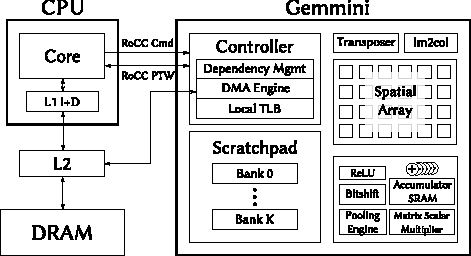
\includegraphics[width=0.8\textwidth]{Gemmini_ArchitectureOverview.pdf}
    \caption{High-level overview of the \texttt{Gemmini} accelerator integrated with a host CPU (\texttt{Rocket Core}) and system memory hierarchy.}
    \label{fig:gemmini_soc_overview}
\end{figure}

\subsection{Systolic Array (Spatial Array)}
\label{subsec:gemmini_systolic_array}
The heart of \texttt{Gemmini} is its systolic array, also referred to as a spatial array. This array consists of a grid of Processing Elements (\texttt{PEs}), each capable of performing Multiply-Accumulate (\texttt{MAC}) operations. The systolic array is highly configurable in terms of:
\begin{itemize}
    \item \textbf{Dimensions:} The number of rows and columns in the \texttt{PE} grid (e.g., 16x16, 32x32).
    \item \textbf{Dataflow:} \texttt{Gemmini} supports different dataflow strategies, primarily Weight Stationary (\texttt{WS}) and Output Stationary (\texttt{OS}). In \texttt{WS} dataflow, weights are pre-loaded into the \texttt{PEs} and remain stationary while input activations stream through. In \texttt{OS} dataflow, partial sums of the output activations remain stationary within the \texttt{PEs} while inputs and weights are streamed. The choice of dataflow can significantly impact performance and energy efficiency depending on the DNN layer characteristics and memory access patterns.
    \item \textbf{Pipelining:} The degree of pipelining within the array and \texttt{PEs} affects the clock speed and throughput.
\end{itemize}
This configurable systolic array allows \texttt{Gemmini} to efficiently execute dense matrix multiplications, which are fundamental operations in many DNN layers, particularly fully connected and convolutional layers (often after an \texttt{im2col} transformation).

\subsection{Local Scratchpad Memory}
\label{subsec:gemmini_scratchpad}
\texttt{Gemmini} includes a dedicated on-chip scratchpad memory. This is a software-managed SRAM used for staging input activations, weights, and intermediate feature maps close to the systolic array.
\begin{itemize}
    \item \textbf{Purpose:} Reduces the latency and energy consumption associated with fetching data from or writing data to higher levels of the memory hierarchy (e.g., L2 cache or main memory/DRAM).
    \item \textbf{Configurability:} The capacity of the scratchpad (e.g., 256 KB) and the number of banks it is divided into are configurable parameters. Multiple banks allow for parallel access, potentially improving bandwidth.
\end{itemize}
Efficient management of the scratchpad memory is crucial for achieving high utilization of the systolic array.

\subsection{Accumulator Memory}
\label{subsec:gemmini_accumulator}
Separate from the main scratchpad, \texttt{Gemmini} features an accumulator memory.
\begin{itemize}
    \item \textbf{Purpose:} Stores the partial sums generated by the \texttt{MAC} operations in the systolic array. These sums are typically of higher precision than the input data types to maintain accuracy during accumulation.
    \item \textbf{Configurability:} The capacity and banking of the accumulator memory are also configurable.
\end{itemize}
After accumulation, the results can be scaled, quantized, and passed through activation functions before being written back to the scratchpad or main memory.

\subsection{Controller and DMA Engine}
\label{subsec:gemmini_controller_dma}
A dedicated controller manages the overall operation of the \texttt{Gemmini} accelerator. It decodes instructions received from the host CPU via the \texttt{RoCC} interface and orchestrates the data movements and computations.
\texttt{Gemmini} incorporates a Direct Memory Access (\texttt{DMA}) engine responsible for:
\begin{itemize}
    \item Transferring data between the external memory (L2 cache/DRAM) and the internal scratchpad memory.
    \item Moving data between the scratchpad and the accumulator memory.
\end{itemize}
The DMA engine operates in parallel with the systolic array computations to hide memory latency.

\subsection{Optional Functional Units}
\label{subsec:gemmini_optional_units}
\texttt{Gemmini} can be configured with several optional hardware units to accelerate common non-GEMM (General Matrix Multiply) DNN operations. These include:
\begin{itemize}
    \item \textbf{Activation Functions:} Hardware support for functions like ReLU.
    \item \textbf{Pooling Layers:} Max-pooling or average-pooling operations.
    \item \textbf{Normalization/Scaling:} For quantizing or scaling results.
    \item \textbf{Transposer:} For matrix transposition if needed by the dataflow or layer.
    \item \textbf{Im2col Unit:} A dedicated unit to perform the \texttt{im2col} transformation (converting image patches into columns for convolution via GEMM) directly in hardware, which can offload the host CPU.
\end{itemize}
These units can be included or excluded during the \texttt{Gemmini} generation process (elaboration time) based on target application requirements, allowing for trade-offs between area/flexibility and performance.

\subsection{Virtual Address Translation Support}
\label{subsec:gemmini_vat}
To operate within a system using virtual memory (like Linux-based SoCs), \texttt{Gemmini}'s DMA needs to translate virtual addresses (used by software) to physical addresses (used by hardware).
\begin{itemize}
    \item \texttt{Gemmini} typically utilizes the host CPU's Page Table Walker (\texttt{PTW}) for this translation.
    \item It can also be configured with its own local Translation Lookaside Buffer (\texttt{TLB}) to cache recent address translations, reducing the latency of PTW lookups. The capacity and hierarchy (e.g., L2 TLB) of Gemmini's TLB are configurable.
\end{itemize}

\section{Gemmini Integration as a RoCC Accelerator}
\label{sec:gemmini_rocc_integration}

As discussed in Chapter \ref{chap:MultiCoreRISCVSystem}, the \texttt{Chipyard} framework supports the integration of custom accelerators via the \texttt{RoCC} interface. \texttt{Gemmini} is designed as such a \texttt{RoCC} accelerator, enabling tight coupling with a \texttt{RISC-V} core like \texttt{Rocket}.

\begin{figure}[h!]
    \centering
    % You can use a diagram similar to slide 43 of Gemmini Introduction.pdf
    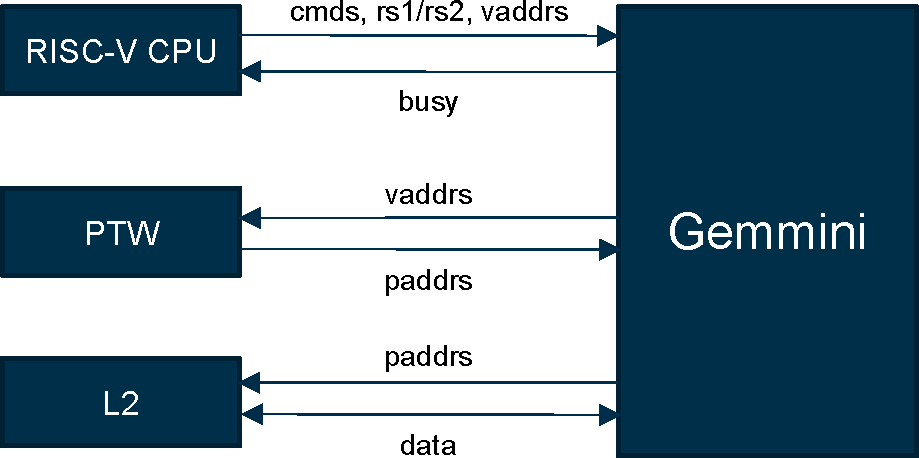
\includegraphics[width=0.7\textwidth]{Gemmini_LowLevel_withCPU.pdf}
    \caption{Conceptual diagram of the \texttt{Gemmini} RoCC interface with the host CPU (\texttt{RISC-V CPU}), PTW, and L2 Cache/System Memory.}
    \label{fig:gemmini_rocc_interface}
\end{figure}

The interaction involves:
\begin{enumerate}
    \item \textbf{Custom Instructions:} The host CPU (e.g., \texttt{Rocket Core}) issues custom \texttt{RISC-V} instructions to \texttt{Gemmini}. These instructions are part of the reserved \texttt{RoCC} opcode space. The format is typically `customX rd, rs1, rs2, funct7`, where `X` selects one of up to four \texttt{RoCC} units, `rd` is the destination CPU register (for status or small results), `rs1` and `rs2` are source CPU registers (often holding data or pointers to data/configuration structures), and `funct7` provides further instruction differentiation for \texttt{Gemmini}.
    \item \textbf{Operand Passing:} Operands from the CPU's register file (`rs1`, `rs2`) are passed to \texttt{Gemmini}. These can include configuration parameters, memory addresses for DMA, or scalar values.
    \item \textbf{Status Reporting:} \texttt{Gemmini} can signal its status (e.g., `busy`) back to the CPU. The CPU can poll this status or use fences for synchronization.
    \item \textbf{Memory Access:} For bulk data, \texttt{Gemmini}'s DMA engine directly accesses the memory system (L2 cache, DRAM) via the \texttt{TileLink} bus, using physical addresses obtained after translation by the PTW. This data path bypasses the CPU's core execution pipeline for high-bandwidth transfers.
\end{enumerate}

\texttt{Gemmini} employs decoupled access-execute pipelines, often managed through separate instruction queues for load (memory to scratchpad), execute (computation on scratchpad data), and store (scratchpad to memory) operations. This decoupling allows for overlapping computation with data movement, enhancing performance.

\section{Gemmini Programming Model}
\label{sec:gemmini_programming_model}
\texttt{Gemmini} supports a multi-level programming model, catering to different needs from direct hardware control to higher-level abstractions.

\begin{figure}[h!]
    \centering
    % You can use a diagram similar to slide 32 of Gemmini Introduction.pdf
    % \includegraphics[width=0.6\textwidth]{placeholder_gemmini_prog_model.png}
    \caption{Layered programming model for \texttt{Gemmini}.}
    \label{fig:gemmini_prog_model}
\end{figure}

\subsection{Low-Level: Gemmini ISA (RoCC Instructions)}
\label{subsec:gemmini_low_level_isa}
At the lowest level, \texttt{Gemmini} is controlled by its custom \texttt{RoCC} instruction set. These instructions are typically wrapped in C preprocessor macros or inline assembly for easier use from C/C++ code. Key instruction categories include:
\begin{itemize}
    \item \textbf{Configuration Instructions:} To set up \texttt{Gemmini}'s internal state, data types, addresses for DMA, and activation functions.
    \item \textbf{Data Movement Instructions (`mvin`, `mvout`):}
        \begin{itemize}
            \item `\texttt{mvin}` (move in): Transfers data from main memory to \texttt{Gemmini}'s scratchpad.
            \item `\texttt{mvout}` (move out): Transfers data from \texttt{Gemmini}'s scratchpad/accumulator to main memory. It can also apply activation functions and pooling during this process.
        \end{itemize}
    \item \textbf{Execution Instructions (`preload`, `compute`):}
        \begin{itemize}
            \item `\texttt{preload}`: Loads stationary data (e.g., weights for WS dataflow, or partial sums for OS dataflow) into the systolic array's internal registers.
            \item `\texttt{compute}`: Initiates a matrix multiplication using data already preloaded into the array and data streamed from the scratchpad.
        \end{itemize}
\end{itemize}
\texttt{Gemmini} also offers "complex" instructions like `\texttt{loop\_matmul}` or `\texttt{loop\_conv}` which encapsulate common looping structures and data tiling, unrolled by hardware Finite State Machines (\texttt{FSMs}). These can simplify programming for common layer types by abstracting scratchpad management to some extent, enabling dynamic scheduling and potentially better overlap of load/execute/store operations.

\subsection{Mid-Level: Hand-Tuned C Library}
\label{subsec:gemmini_mid_level_library}
To abstract the complexities of direct ISA programming, \texttt{Gemmini} provides a C library (often through `\texttt{gemmini.h}`). This library offers functions for common DNN operations, such as:
\begin{itemize}
    \item `\texttt{tiled\_matmul}`: Performs tiled matrix multiplication, handling data movement and computation for larger matrices than can fit in the scratchpad at once.
    \item `\texttt{tiled\_conv}`: Performs tiled convolution (often using \texttt{im2col} and \texttt{tiled\_matmul} internally).
    \item Functions for residual additions, pooling, etc.
\end{itemize}
These library functions utilize heuristics for loop tiling and data movement to maximize buffer usage and systolic array utilization. They rely on a configuration header file (e.g., `\texttt{gemmini\_params.h}`) that reflects the specific hardware parameters of the generated \texttt{Gemmini} instance (e.g., array dimensions, scratchpad size). This allows the same C code to be used with different \texttt{Gemmini} hardware configurations.

\subsection{High-Level: Compiler Support (Conceptual)}
\label{subsec:gemmini_high_level_compiler}
While not the primary focus of this thesis's implementation, the \texttt{Gemmini} ecosystem aims to support higher-level compilation flows. This involves tools that can take DNN models described in frameworks like ONNX (Open Neural Network Exchange) or TensorFlow Lite and compile them down to \texttt{Gemmini} instructions, potentially leveraging the mid-level C library or directly generating low-level ISA calls. This further simplifies the deployment of DNNs on \texttt{Gemmini}-accelerated SoCs.

\section{Gemmini Configuration in This Thesis}
\label{sec:gemmini_configuration_thesis}

The \texttt{Gemmini} accelerator integrated into the SoC for this thesis is based on a specific configuration suitable for the target AI applications. Within the \texttt{Chipyard} framework, configurations are typically defined in Scala. A common starting point for a single \texttt{Rocket Core} with \texttt{Gemmini} is the `\texttt{TutorialGemminiRocketConfig}` or a derivative.

For this project, the \texttt{Gemmini} instance was configured with [**Specify key parameters here: e.g., systolic array dimensions (e.g., 16x16), scratchpad size (e.g., 256KB), accumulator size (e.g., 64KB), dataflow type (e.g., Weight Stationary), whether the hardware im2col unit was included, etc. These details should come from your actual implementation choices.**]. These parameters were chosen to balance performance for target DNN workloads with the resource constraints typical of an FPGA-based or academic ASIC implementation. The detailed performance implications of these choices will be explored in subsequent chapters.

The integration follows the standard \texttt{RoCC} methodology provided by \texttt{Chipyard}, ensuring that \texttt{Gemmini} coexists with the \texttt{Rocket Core}, shares the memory system hierarchy, and can be programmed using custom \texttt{RISC-V} instructions dispatched to its \texttt{RoCC} slot.

\section{Summary}
\label{sec:gemmini_summary}
\texttt{Gemmini} serves as the core computational engine for DNN acceleration in the SoC designed for this thesis. Its flexible, generator-based architecture allows for tailoring to specific needs, and its integration as a \texttt{RoCC} accelerator provides a tight coupling with the host \texttt{RISC-V} processor. The multi-level programming model offers pathways for both detailed hardware control and higher-level application development. By leveraging \texttt{Gemmini} within the \texttt{Chipyard} framework, this thesis aims to demonstrate an effective approach to building and evaluating specialized hardware for AI applications.